\chapter{Draw diagrams}

You can find a lot of examples here: \url{http://www.tn-home.de/TUGDD/Stuff/TikZ_final.pdf}

\section{simple}

\begin{figure}[h!]

\begin{tikzpicture}
	\path            (0,0) circle (2ex);
	\path[draw]      (1,0) circle (2ex);
	\path[fill]      (2,0) circle (2ex);
	\path[fill=yellow,draw=red] (3,0) circle (2ex);
	\path[clip]         (4,0) circle (2ex);
	\fill[color=orange] (3.5,-.5) rectangle (4.5,.5);
\end{tikzpicture}
\end{figure}

\section{inline graphic}
This is an inline graphic \tikz \draw[fill=orange] (0,0) circle (1ex);

\section{not so simple}
\begin{figure}[h!]
% Its better to put them in a figure
	\begin{center}
		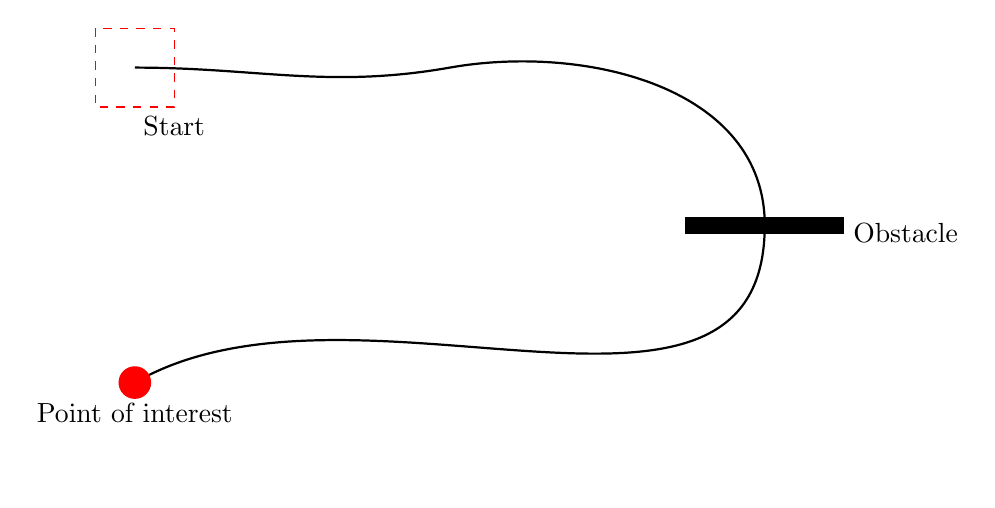
\begin{tikzpicture}
		% Draws a rectangle at -2.5,2.5 with the dimensions -1.5,1.5 and prints a black Start below 
		\draw [red,dashed] (-2.5,2.5) rectangle (-1.5,1.5) node [black,below] {Start};
		% Draws a thick line from -2,2 to 2,2 with in out angle of 0 and an in angle of 190 degrees
		\draw [thick] (-2,2)
		to [out=0,in=190] (2,2)
		to [out=10,in=90] (6,0) 
		to [out=-90,in=30] (-2,-2);    
		\draw [fill] (5,0.1) rectangle (7,-0.1) node [black,right] {Obstacle}; % Draws another rectangle
		\draw [red,fill] (-2,-2) circle [radius=0.2] node [black,below=4] {Point of interest}; % Draws a circle
		\end{tikzpicture}
		\caption{Example graphic made with tikz.}
	\end{center}
\end{figure}

\section{GNUPlot}

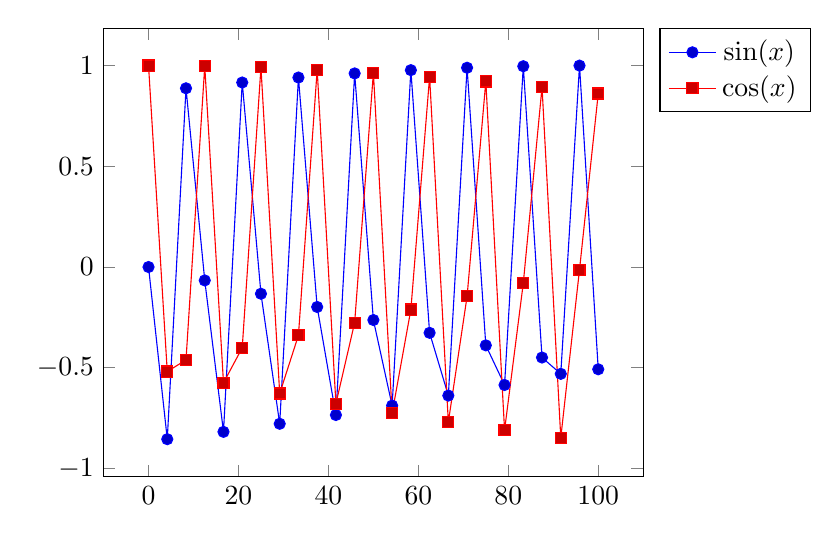
\begin{tikzpicture}
\begin{axis}[domain=0:100,legend pos=outer north east]
	\addplot {sin(deg(x))};
	\addplot {cos(deg(x))};
	\legend{$\sin(x)$,$\cos(x)$}
\end{axis}
\end{tikzpicture}